\part{Esposizione}
\chapter{Architettura Android}

\epigraph{Fully understanding the internals of Android's system services is like trying to swallow a whale}%
{K. Yaghmour\\Embedded Android}

\minitoc\mtcskip



\begin{figure}[thp]
\centering
\subfloat[][\textit{Visione High-Level dell'Architettura di Android. \url{http://androidteam.googlecode.com/files/system-architecture.jpg}}]{\label{subfig:googleaview}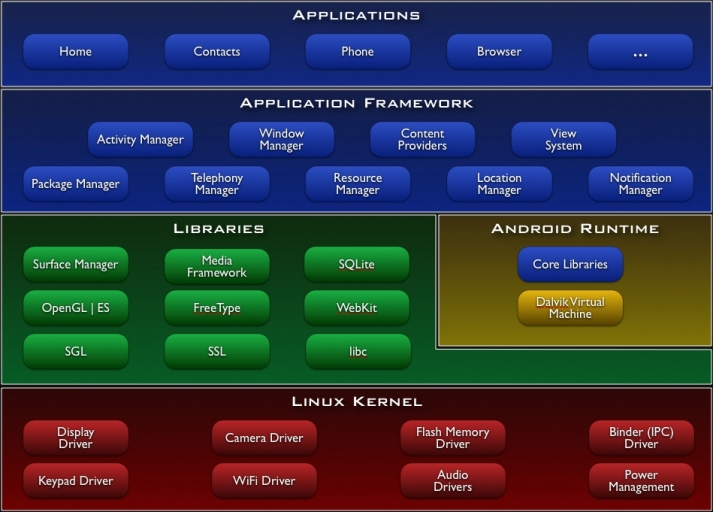
\includegraphics[scale=0.5]{img/system-architecture.jpg}}\\
\subfloat[][\textit{Visione Low-Level dell'Architettura di Android. \parencite{libro:embedded}}]{\label{subfig:embedaview}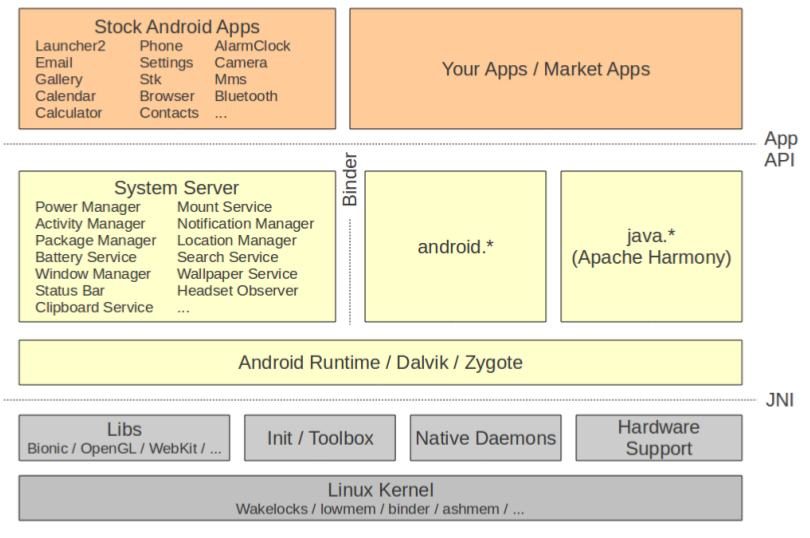
\includegraphics[scale=0.5]{img/embed/arch.png}}\\
\caption{Vari livelli della visualizzazione dell'Architettura di Android (1).}
\label{fig:androidarchview}
\end{figure}
\textit{Lo scopo di questo capitolo è quello di dettagliare come avvengano le interazioni
all'interno del sistema operativo, allo scopo di mostrare nei capitoli successivi
come sia possibile l'interazione tra codice nativo e servizi di sistema.}

In genere si descrive l'architettura di Android come quella dell'immagine fornita
dalla stessa Google (v. Figura \subref{subfig:googleaview} \vref{fig:androidarchview}), 
anche se questa visualizzazione esclude del tutto dalla gerarchia le applicazioni
native. Quest'immagine non evidenzia infatti l'effettiva architettura del sistema
operativo, ma ne descrive la gerarchia logica-funzionale, necessaria allo sviluppatore
Android Java per gestire unicamente l'interazione tra le applicazioni
(il primo strato in alto) ed i servizi (quelli immediatamente sotto).
Nell'immagine non viene affatto mostrato come questo meccanismo avvenga: ciò è permesso
dall'esistenza del \textbf{Binder}, che tuttavia verrà descritto in 
seguito nel dettaglio; per ora è sufficiente sapere che questo meccanismo implementa
il sistema utilizzato da Android per effettuare l'IPC tra
programmi e servizi.

Come dice lo stesso \parencite{art:notdroid}, Android è di fatti una versione
modificata del Kernel Linux, 
che ha subito sostanziali modifiche, quali l'incorporazione di \textit{udev} dentro
ad \textit{init}. È stato inoltre sovrapposto uno strato di servizi
 detto \textit{Android Middleware}, scritto sia in Java, sia in C++ sia in C, 
allo scopo di implementare nuove funzionalità (e, nel contempo, introdurre 
ulteriori limitazioni nell'utilizzo del dispositivo\footnote{Avrò modo di 
dimostrare questa tesi più avanti nella mia trattazione, come a conclusione
del corrente capitolo.
}).

\begin{figure}[thp]
\centering
\subfloat[][\textit{Visione dello stack di Android dal punto di vista dell'interazione tra strati architetturali. \parencite{site:marakRemixing}}]{\label{subfig:marakiview}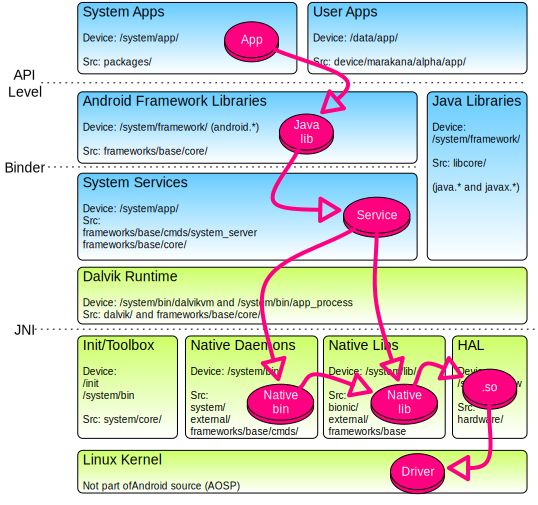
\includegraphics[scale=0.5]{img/marak/android_interaction}}\\
\caption{Vari livelli della visualizzazione dell'Architettura di Android (2).}
\label{fig:androidarchviewtwo}
\end{figure}

Come mostra il livello di strutturazione del sorgente proposto in Figura \subref{subfig:embedaview} \vref{fig:androidarchview},
le applicazioni native sono effettivamente situate allo stesso livello delle
altre applicazioni di sistema, in quanto anch'esse debbono scontrarsi con 
\textit{Android Middleware},
che regola anche il funzionamento degli stessi applicativi. 

Come daltronde messo in luce in \parencite{tesi:nexus}, è sempre a livello Java
che avviene la limitazione nella selezione dell'interfaccia di rete di default, non
rendendo possibile, a meno di modifica dello strato dei servizi, l'utilizzo contemporaneo di due interfacce:
una visione generale di questo meccanismo, suggerirebbe 
la ricompilazione di alcune librerie già disponibili in Android allo scopo di
bypassare suddetti controlli.
Una prima \textit{overview} dell'interazione dei vari strati occorrente nell'esecuzione
di applicativi Java è evidenziato in Figura \subref{subfig:marakiview} 
\vref{fig:androidarchviewtwo},
che ben descrive la situazione generale del comportamento del sistema operativo.

